\documentclass[11pt,letterpaper]{article}

\usepackage{graphicx}
\usepackage[margin=1in]{geometry}
\usepackage{amsmath}
\usepackage[T1]{fontenc}
\usepackage[utf8]{inputenc}
\usepackage{authblk}
\usepackage{fancyhdr}
\usepackage{lastpage}
\usepackage[parfill]{parskip}
\usepackage{subcaption}

\pagestyle{fancyplain}

% Headers
\lhead{}
\chead{}
\rhead{}

% Footers
\lfoot{}
\cfoot{}
\rfoot{\footnotesize Page \thepage\ of \pageref{LastPage}}

\renewcommand{\headrulewidth}{0.0pt} % No header rule
\renewcommand{\footrulewidth}{0.4pt} % Thin footer rule

\title{Research Proposal: Consensus Shootout by Simulation}
\date{April 29, 2016}
\author[ ]{Benjamin Bengfort}
\author[ ]{Pete Keleher}
\affil[ ]{Department of Computer Science}
\affil[ ]{University of Maryland}
\affil[ ]{\textit{\{bengfort,keleher\}@cs.umd.edu}}

\begin{document}

\maketitle

\begin{abstract}
We propose to leverage our simulation framework created for the purpose of studying federated consistency, to review and evaluate multiple popular consensus algorithms. In our review, we will briefly describe each algorithm along with a message flow diagram outlining how many steps are required for consensus decisions. We will compare and contrast the algorithms experimentally in simulation by measuring messages per decision, latency, and correctness. Finally we will visualize the behavior of each algorithm using an interactive JavaScript web application. Through this work we hope not only to compare consensus algorithms but also create reference implementations as well as a teaching tool for use at the University of Maryland.
\end{abstract}

\section*{Introduction}

There are a myriad of algorithms designed to coordinate the replication of a linearizable sequence of events, generally referred to as distributed consensus. Many of these algorithms extend the Paxos protocol \cite{lamport_paxos_2001}, notorious for its difficulty in implementation \cite{chandra_paxos_2007} and understandability \cite{ongaro_search_2014}, to provide faster or more efficient consensus decisions. Although Paxos has been implemented in real systems \cite{bolosky_paxos_2011,burrows_chubby_2006}, many of its descendants are either not publicly available or provide reference implementations that are open to interpretation.

Further complicating matters is the general difficulty reproducing results for systems; not only do the algorithms have to be implemented from their descriptions in papers, so to does the experimental setup have to be replicated. This challenges reviewers in both time and expense; as well as limits pedagogical opportunities. In 2014, Collberg et al. studied the reproducibility of 613 papers from eight ACM conferences and determined that 308 (50\%) of papers were not reproducible after searching for GitHub, Sourceforge, or BitBucket repositories and then emailing the authors for more information \cite{collberg_measuring_2014}. Efforts to encourage reproducibility through community exhortation \cite{kovacevic_how_2007} or even by grand challenges \cite{van_gorp_share_2011} have fallen short.

The implementation of the Raft algorithm \cite{ongaro_search_2014}, however, may have changed things for distributed consensus. Raft became very popular after its publication, and in fact there are now at least 76 reference implementations in a variety of programming languages. In terms of reproducibility, Howard et al. used a discrete event simulation to easily create an environment with which to test the experiments designed by Ongaro and Ousterhout \cite{howard_raft_2015}. In terms of pedagogy, a number of tools exist for explaining the Raft algorithm using interactive JavaScript visualizations \cite{johnson_secret_2014,ongaro_raft_2015}.

We propose to extend the work done by Howard et al. by similarly creating a general consensus simulator, which we will make open source and available for consensus experiments. The simulator will contain two parts: an event based simulator that can exercise trace data into a consensus algorithm, measure its performance, and verify its correctness; as well as a visual front-end that will demonstrate how the consensus algorithm responds to reads and writes in the system. We will then utilize the simulator to study several distributed consensus algorithms, verify their results and compare them in a controlled environment.

\section*{Proposal}

In this section we will describe the two distinct parts of our proposal: the study we propose to undertake, and the simulator we hope to extend for use in our study. The goals for both the study and the simulator are as follows:

\begin{enumerate}
    \setlength\itemsep{-0.75em}
    \item Survey current distributed consensus algorithms.
    \item Measure, validate, and compare performance and correctness for those algorithms.
    \item Produce a tool that can be used to reproduce and review distributed consensus.
    \item Produce visualizations and products that can be used to teach distributed consensus.
\end{enumerate}

Because work has already been started on the simulator (for a different study), we believe that the primary challenge in this proposal will be the development of any algorithm involved in the study (besides Raft, which has already been implemented).

\subsection*{Study}

We propose to survey at least four distributed consensus algorithms, implement them in simulation, and visualize their behavior. This survey would study the differences in distributed consensus algorithms as well as their relative merits and performance gains. In particular, we propose to look at Multi-Paxos \cite{chandra_paxos_2007}, ePaxos \cite{moraru_there_2013}, Raft \cite{ongaro_search_2014}, Warranties \cite{liu_warranties_2014}, and Mencius \cite{mao_mencius_2008}. If possible, we also propose the study of Fast Paxos \cite{lamport_fast_2006}, Chubby \cite{burrows_chubby_2006}, ZooKeeper \cite{hunt_zookeeper_2010}, and Stellar \cite{mazieres_stellar_2015} as stretch goals.

In the study, we will provide a general description of distributed consensus, including outlining specific assumptions and environments that we will simulate. We will discuss each protocol as concisely as possible, but will particularly include message flow diagrams of each that show how many messages or steps are required for consensus. We will conduct experiments using a simulated network environment and compare and contrast the protocols. Finally, we will use the simulator's front-end JavaScript visualization to demonstrate how each protocol works.

For the experimental study, we will simulate a fixed set of access events (reads/writes) to the cluster. We will measure the total time required to complete the simulation, the number of messages required, the commit and visibility latency, the number of timeouts, and the amount of downtime. We will also verify correctness, in that all replicated nodes maintain the same, consistent ordering at the conclusion of the simulation.

\subsection*{Simulator}

The simulator for this study has already been developed to study federated consensus, and although some work still needs to be done (for example the JavaScript visualization is only 50\% complete) it is in a very good place to undertake this effort. The simulator uses discrete event simulation implemented by the SimPy framework in Python \cite{muller_simpy_2003,muller_simpy_2015}, however real time simulation is also possible.

\begin{figure}
	\centering
    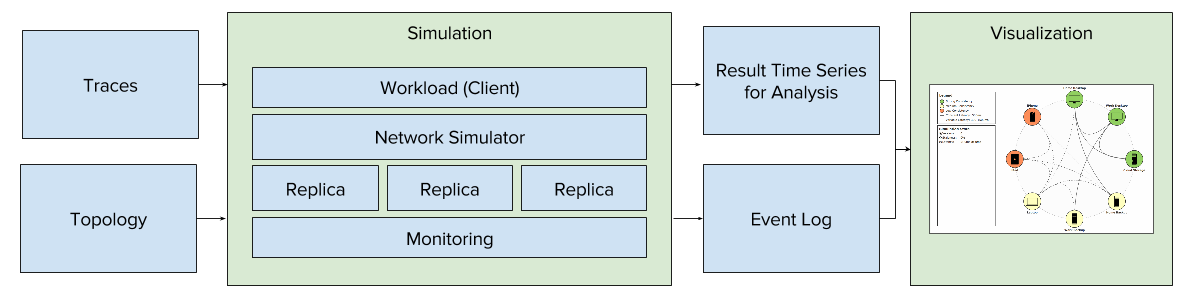
\includegraphics[width=\textwidth]{figures/simulator}
    \caption{\textsf{Component architecture of the distributed consensus simulator that has already been developed.}}
    \label{fig:architecture}
\end{figure}

As shown in Figure \ref{fig:architecture}, the simulator accepts as input a \textit{topology}, specified as a JSON file that determines what nodes are in the system, what consistency levels they're at, and the network latencies between their connections. Additionally the simulator can accept \textit{traces}, a TSV file of fixed event accesses made to each replica in the simulator. The output is a results file formatted as JSON data that includes time series measurements made by the simulation as well as meta data about the configuration of the nodes. Optionally the simulator can also output an event trace which is used to demonstrate behavior through an animation.

Extending the current simulation to include new replica types that implement the various consensus protocol would require subclassing the \texttt{Replica} object and writing event handlers for the various message types and RPCs that need to be implemented.

\section*{Conclusion}

We have proposed a study of multiple distributed consensus protocols that utilizes a currently available simulator to compare and contrast performance. We believe that this survey will be valuable to the systems community both as reference implementations and also as a mechanism to reproduce results. By making the simulator open, we hope to encourage community participation, thereby creating a robust analysis mechanism that is currently unavailable in the field. Moreover, we believe that both the simulator, the survey, and the visualizations will serve as invaluable teaching tools for distributed systems courses.


\bibliographystyle{plain}
\bibliography{paper}

\end{document}
